\ifx\allfiles\undefined
\documentclass[UTF8, a4paper]{ctexart}
\usepackage{geometry}
\geometry{left=1.0cm, right=1.0cm, top=2.0cm, bottom=1.5cm}
\setlength\parskip{0em}

\usepackage{graphicx}
\usepackage{pythonhighlight}
\graphicspath{{img/}}
\bibliographystyle{plain}%指定参考文献的排版样式

\begin{document}
\title{20190529-12 图像语义分割-理解每个像素\cite{slides}}
\author{主持人:程明明(南开大学 )}
\date\today
\maketitle
\tableofcontents
%\else
%\section{20190529-12 图像语义分割-理解每个像素}
\fi

%%%%%%%%%%%%%%%%%%%%%%%%%%%%%%%%%%%%%%%%%%%%%%%%%%%%%%%%%%%%%%%%%%%%%%%%%%%%%%%%
%%% Context for semantic segmentation
%%%%%%%%%%%%%%%%%%%%%%%%%%%%%%%%%%%%%%%%%%%%%%%%%%%%%%%%%%%%%%%%%%%%%%%%%%%%%%%%

\section{Context For Semantic Segmentation}

%%%%%%%%%%%%%%%%%%%%%%%%%%%%%%%%%%%%%%%%%%%%%%%%%%%%%%%%%%%%%%%%%%%%%%%%%%%%%%%%
\subsection{介绍}
\paragraph{报告嘉宾}
俞刚(旷视科技)

\paragraph{报告时间}
2019年5月29日(星期三)晚上20:30(北京时间)

\paragraph{报告题目}Context For Semantic Segmentation

\paragraph{报告人简介}
俞刚博士现为旷视科技研发总监,Detection 组负责人,2014年毕业于新加坡南洋理工大学。
博士毕业后在南洋理工大学从事 research fellow 的研发工作。2014 年底加入旷视科技公司。
其研究方向主要集中在计算机视觉以及机器学习方面,包括物体检测,语义分割,行人姿态估计以及人体动作行为分析。
已经在顶级会议以及期刊上面发表学术论文二十余篇。同时著有书籍一本。
俞刚博士带队参加 2017 COCO+Places 挑战赛获得检测第一名,人体姿态估计第一名;接着带队参加 2018 COCO+Mapillary 挑战赛,获四项第一。
个人主页\cite{Gangyu}。

\paragraph{报告摘要}
Semantic segmentation is a fundamental problem in computer vision society. 
The main challenge is how to deal with the ambiguities when the pixels have similar appearance but different categories. 
Context information is an important cue to deal with the problem. 
In this talk, I will provide four approaches to model the context information in the image, covering the backbone, head and loss in the network design. 
Competitive results have been reported based on the semantic segmentation benchmarks.

%%%%%%%%%%%%%%%%%%%%%%%%%%%%%%%%%%%%%%%%%%%%%%%%%%%%%%%%%%%%%%%%%%%%%%%%%%%%%%%%
\subsection{语义分割概述}

\paragraph{什么是语义分割?}
语义分割实际上是Classification + Localization的任务。与之相关的相关视觉识别的任务有:
\begin{itemize}
    \item Classification 分类
    \item Semantic Segmentation 语义分割
    \item Instance Segmentation 实例分割
    \item Panoptic Segmentation 全景分割
    \item Detection 检测
    \item Keypoint Detection 关键点检测
\end{itemize}

\paragraph{语义分割Pipeline}

语义分割网络主要包括三部分:Backbone、Head和Loss:
$$\fbox{image} \rightarrow \fbox{backbone} \rightarrow \fbox{head + loss} \rightarrow \fbox{segmentation}$$
其中backbone用于下采样进行特征提取,主要有VGG、ResNet、ResNext等;
Loss用于训练的时候进行梯度下降,常见的有L2、交叉熵、softmax等;
Head用于上采样将特征还原到原图大小,常见的有U-shape、4/8-Sampling+Dilation等。

\paragraph{当前的挑战}

当前的语义分割任务最主要的问题就是在\textbf{Speed} 和\textbf{Performance}之间的tradeoff。一般一个网络速度越快性能就越差。
性能包括\textbf{Per-pixel Accuracy}和\textbf{Boundary},前者的衡量指标主要是IoU,侧重于整体;后者侧重边缘细节。

\subsection{语义分割中的Context}
\subsubsection{Backbone}
\paragraph{Motivation}
传统的backbone是用于分类网络的,通过损失分辨率来获得较大的感受野。分割任务要求同时具有分类的精度和定位的准确性,因此需要具有\textbf{大的感受野(Context)和高空间分辨率}。\\
但是大的感受野和高分辨率实际上是矛盾的。要获得大的感受野就需要进行下采样,会损失分辨率;要保持分辨率较高的情况下对于大的物体就无能为力,无法完整捕捉物体信息,而且计算代价也比较大。

{
    {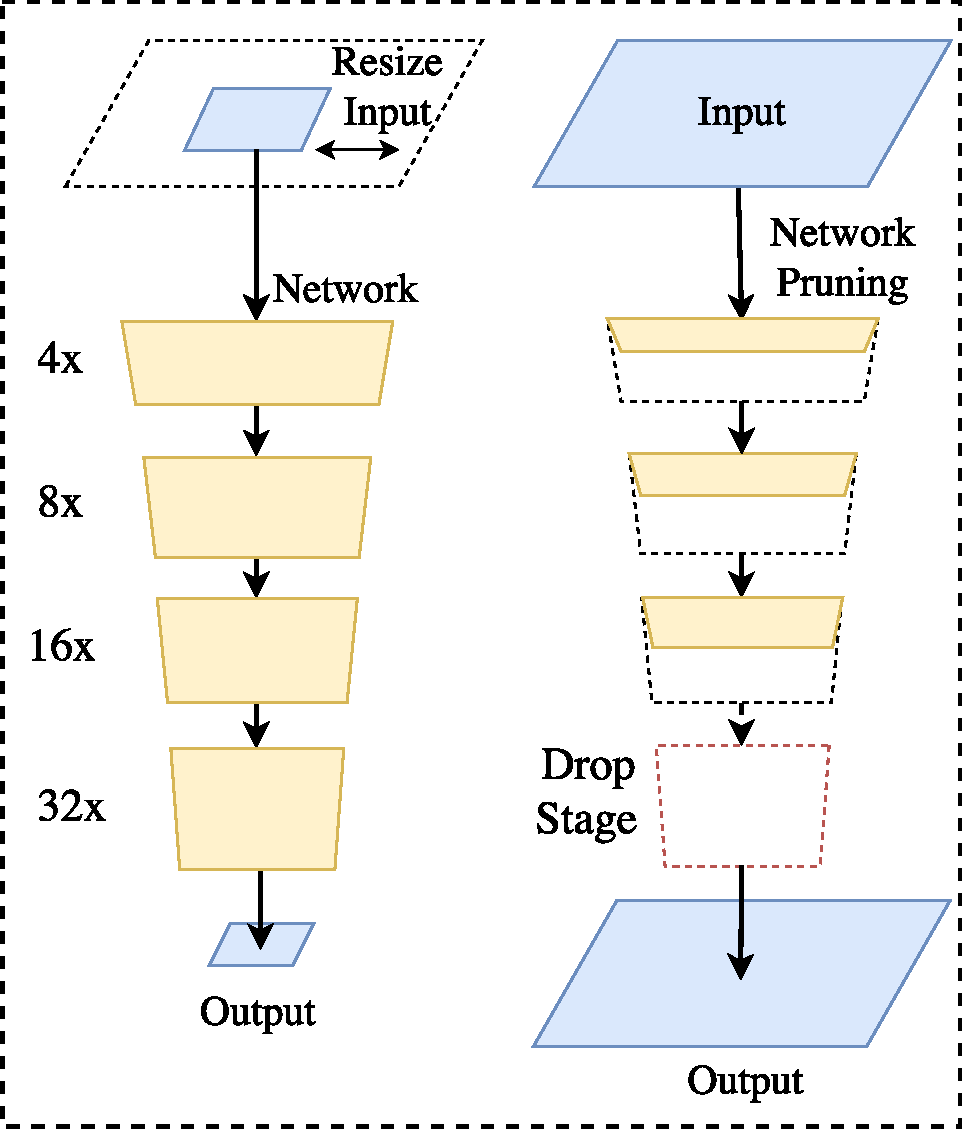
\includegraphics[width=0.3\linewidth]{classic-shape}}
    {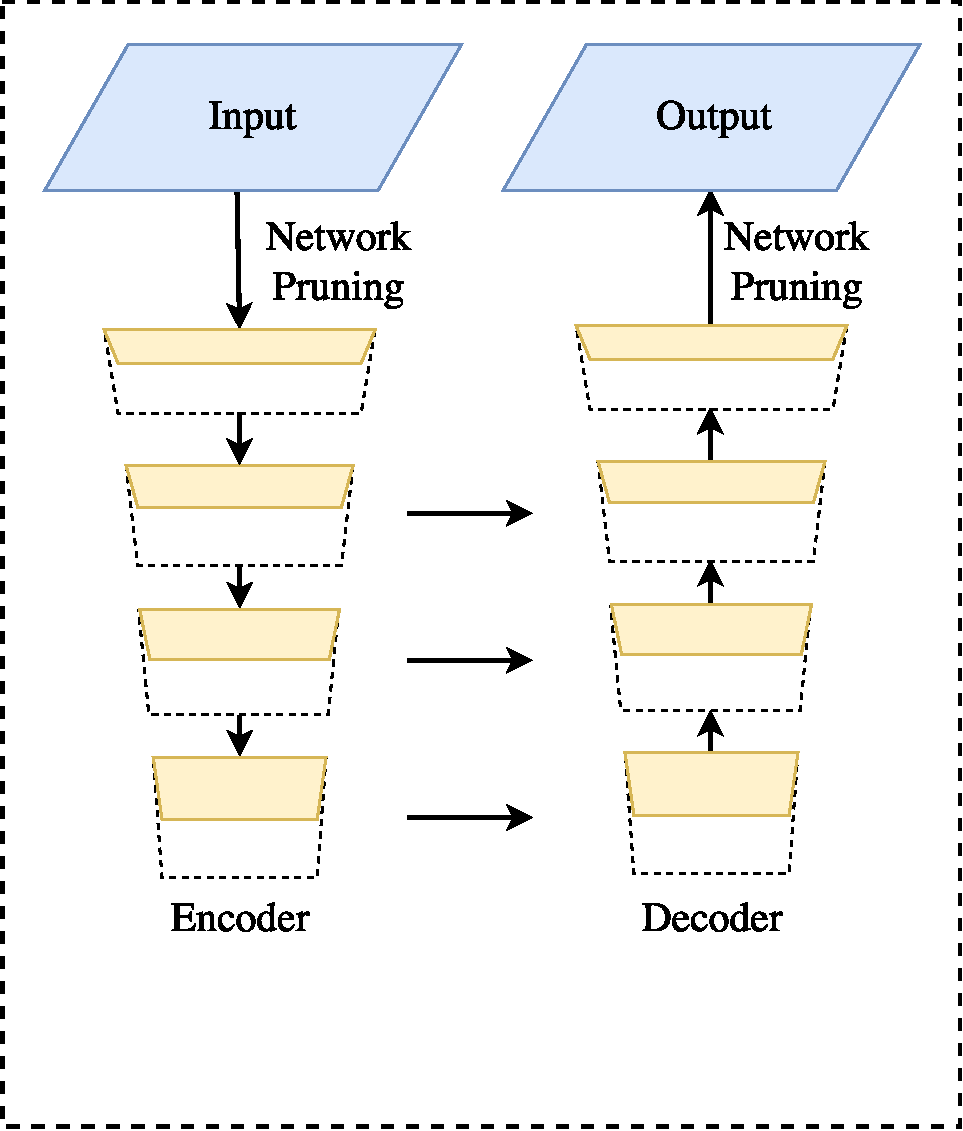
\includegraphics[width=0.3\linewidth]{u-shape}}
    {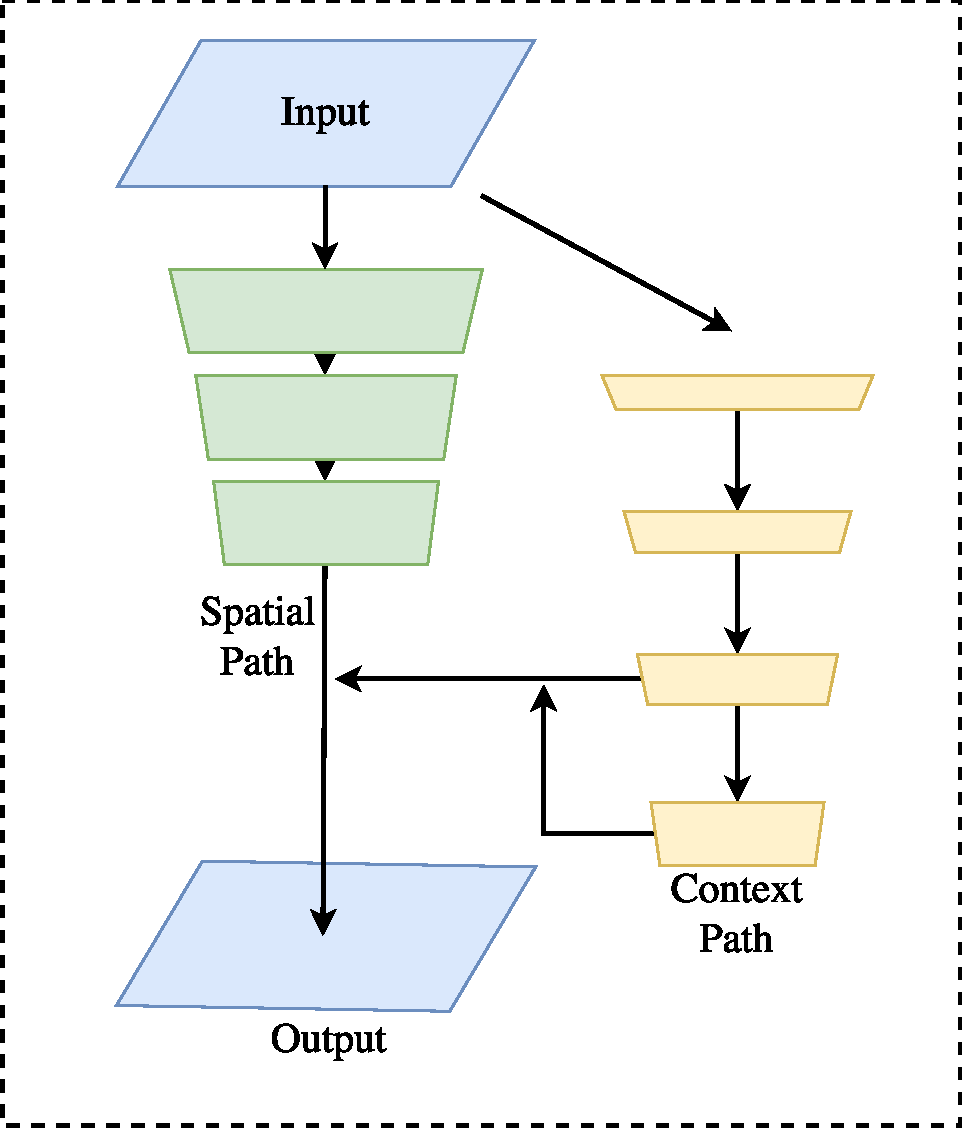
\includegraphics[width=0.3\linewidth]{BiSeNet-shape}}
}

\paragraph{解决方法探索:BiSeNet(ECCV2018)\cite{BiSeNet}}

通过将backbone从原先的一个网络拆分为两个path,分别为spatial path(1/8)和context path(1/32),前者解决分辨率问题,后者解决感受野问题,快速获得较大的感受野,使网络更加轻量级。
两个path通过FFM(特征融合模块)进行融合,然后进行$8\times$上采样。其中Context path还利用ARM(Attention Refinement Module)进行调整。
消融实验结果表明Spatial path、Context path、ARM、FFM和GP(global average pooling)均对结果有一定提升。同时速度也有很大提升。

{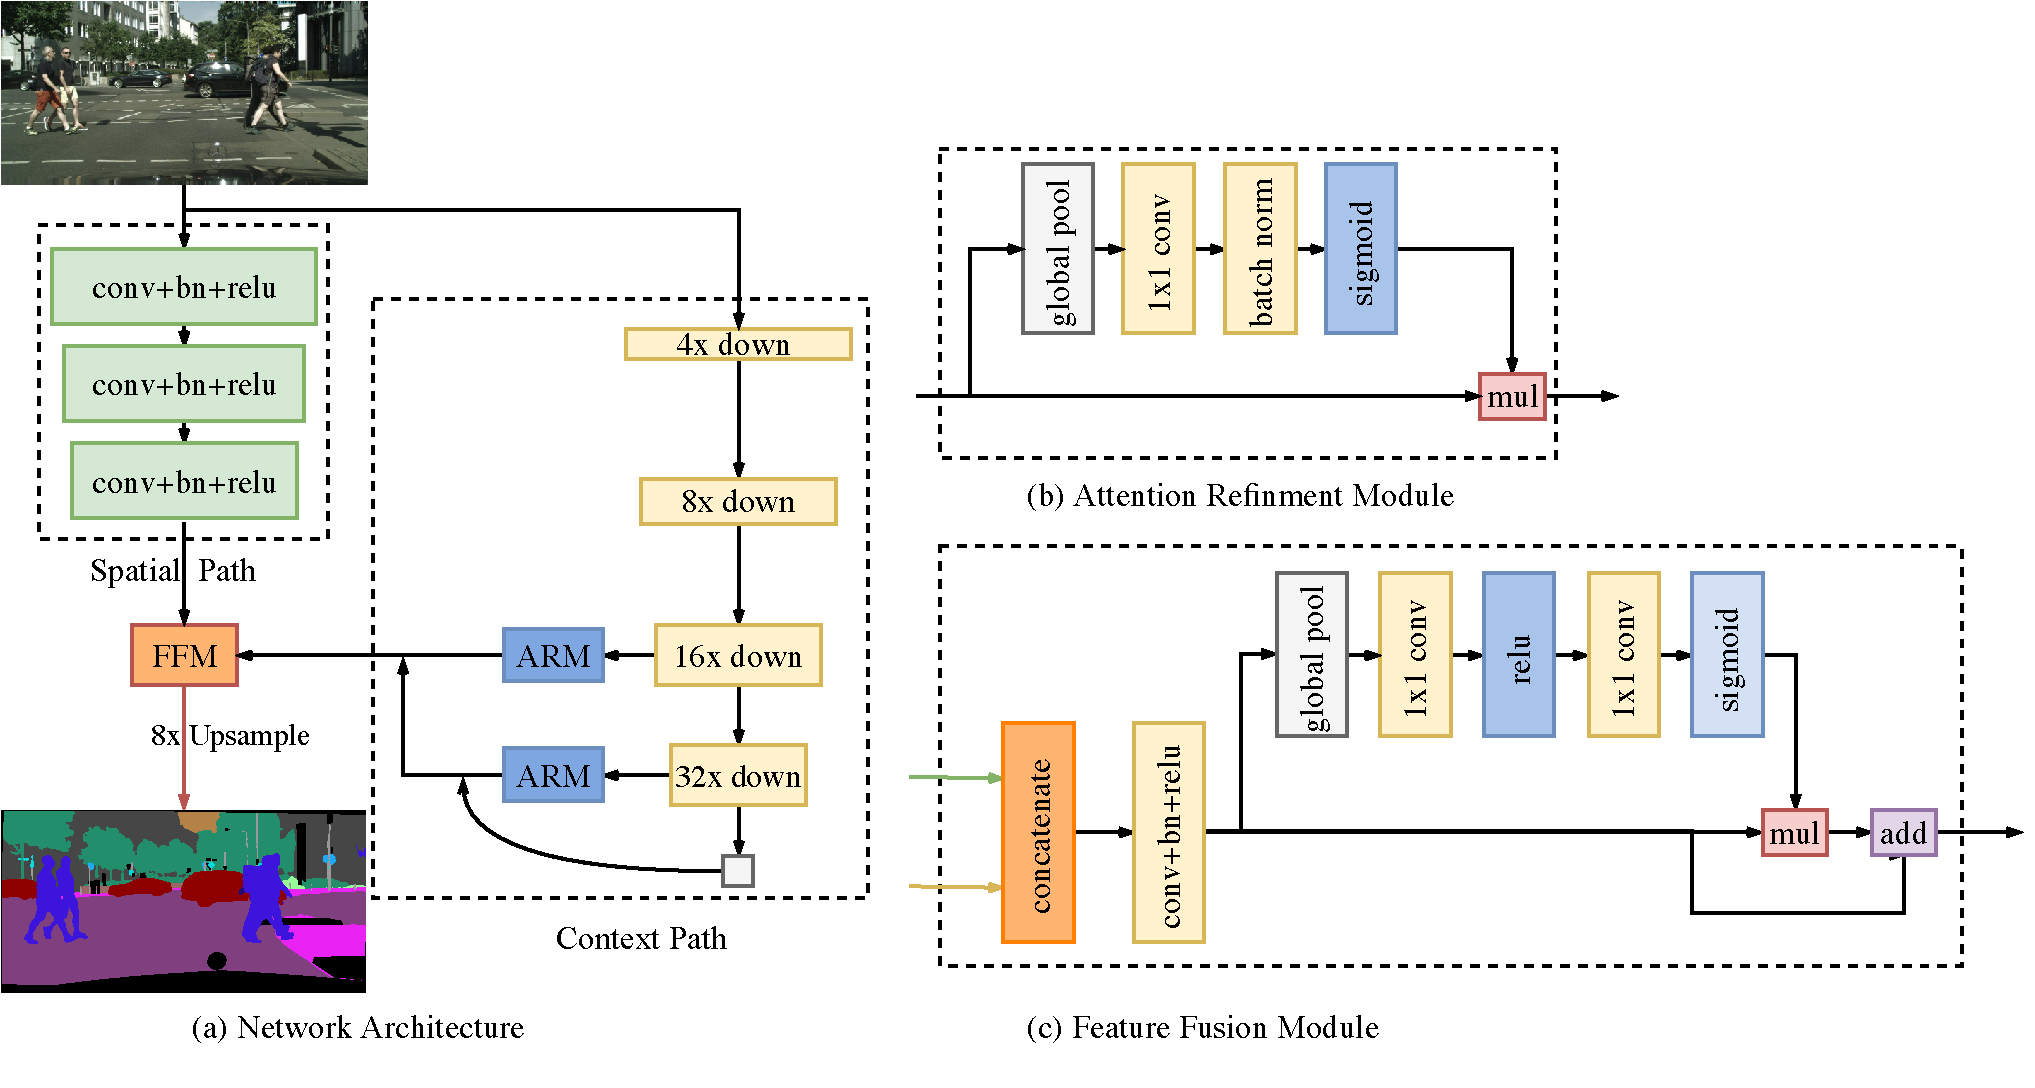
\includegraphics[width=0.95\linewidth]{img/BiSeNet-network}}

\paragraph{总结}
通过backbone中的两路path:context path和spatial path,Context通过感受野进行隐式编码。代码实现在\cite{torchseg_code}。

\subsubsection{Head}

\paragraph{Motivation 1}
大的感受野并不能保证好的边缘结果。在Head部分进行能够速度更快、增大感受野、易于实现。

\paragraph{解决办法探索1:Large Kernel Matters(CVPR2017)\cite{GCN}}
获得大的感受野的同时会使边缘更加模糊。因此在head使用GCN和Boundary Refinement模块,前者使用可分离卷积获得更大感受野,后者使用类残差模块对边缘进行refine。
消融实验结果表明BR确实对于边界有提升,而GCN对内部IoU有较大提升;GCN的kernel size越大IoU越大;同时GCN不能被Conv进行替代,简单的Conv堆叠并不能提升结果。
在backbone中加入GCN对于结果也有微弱提升。

{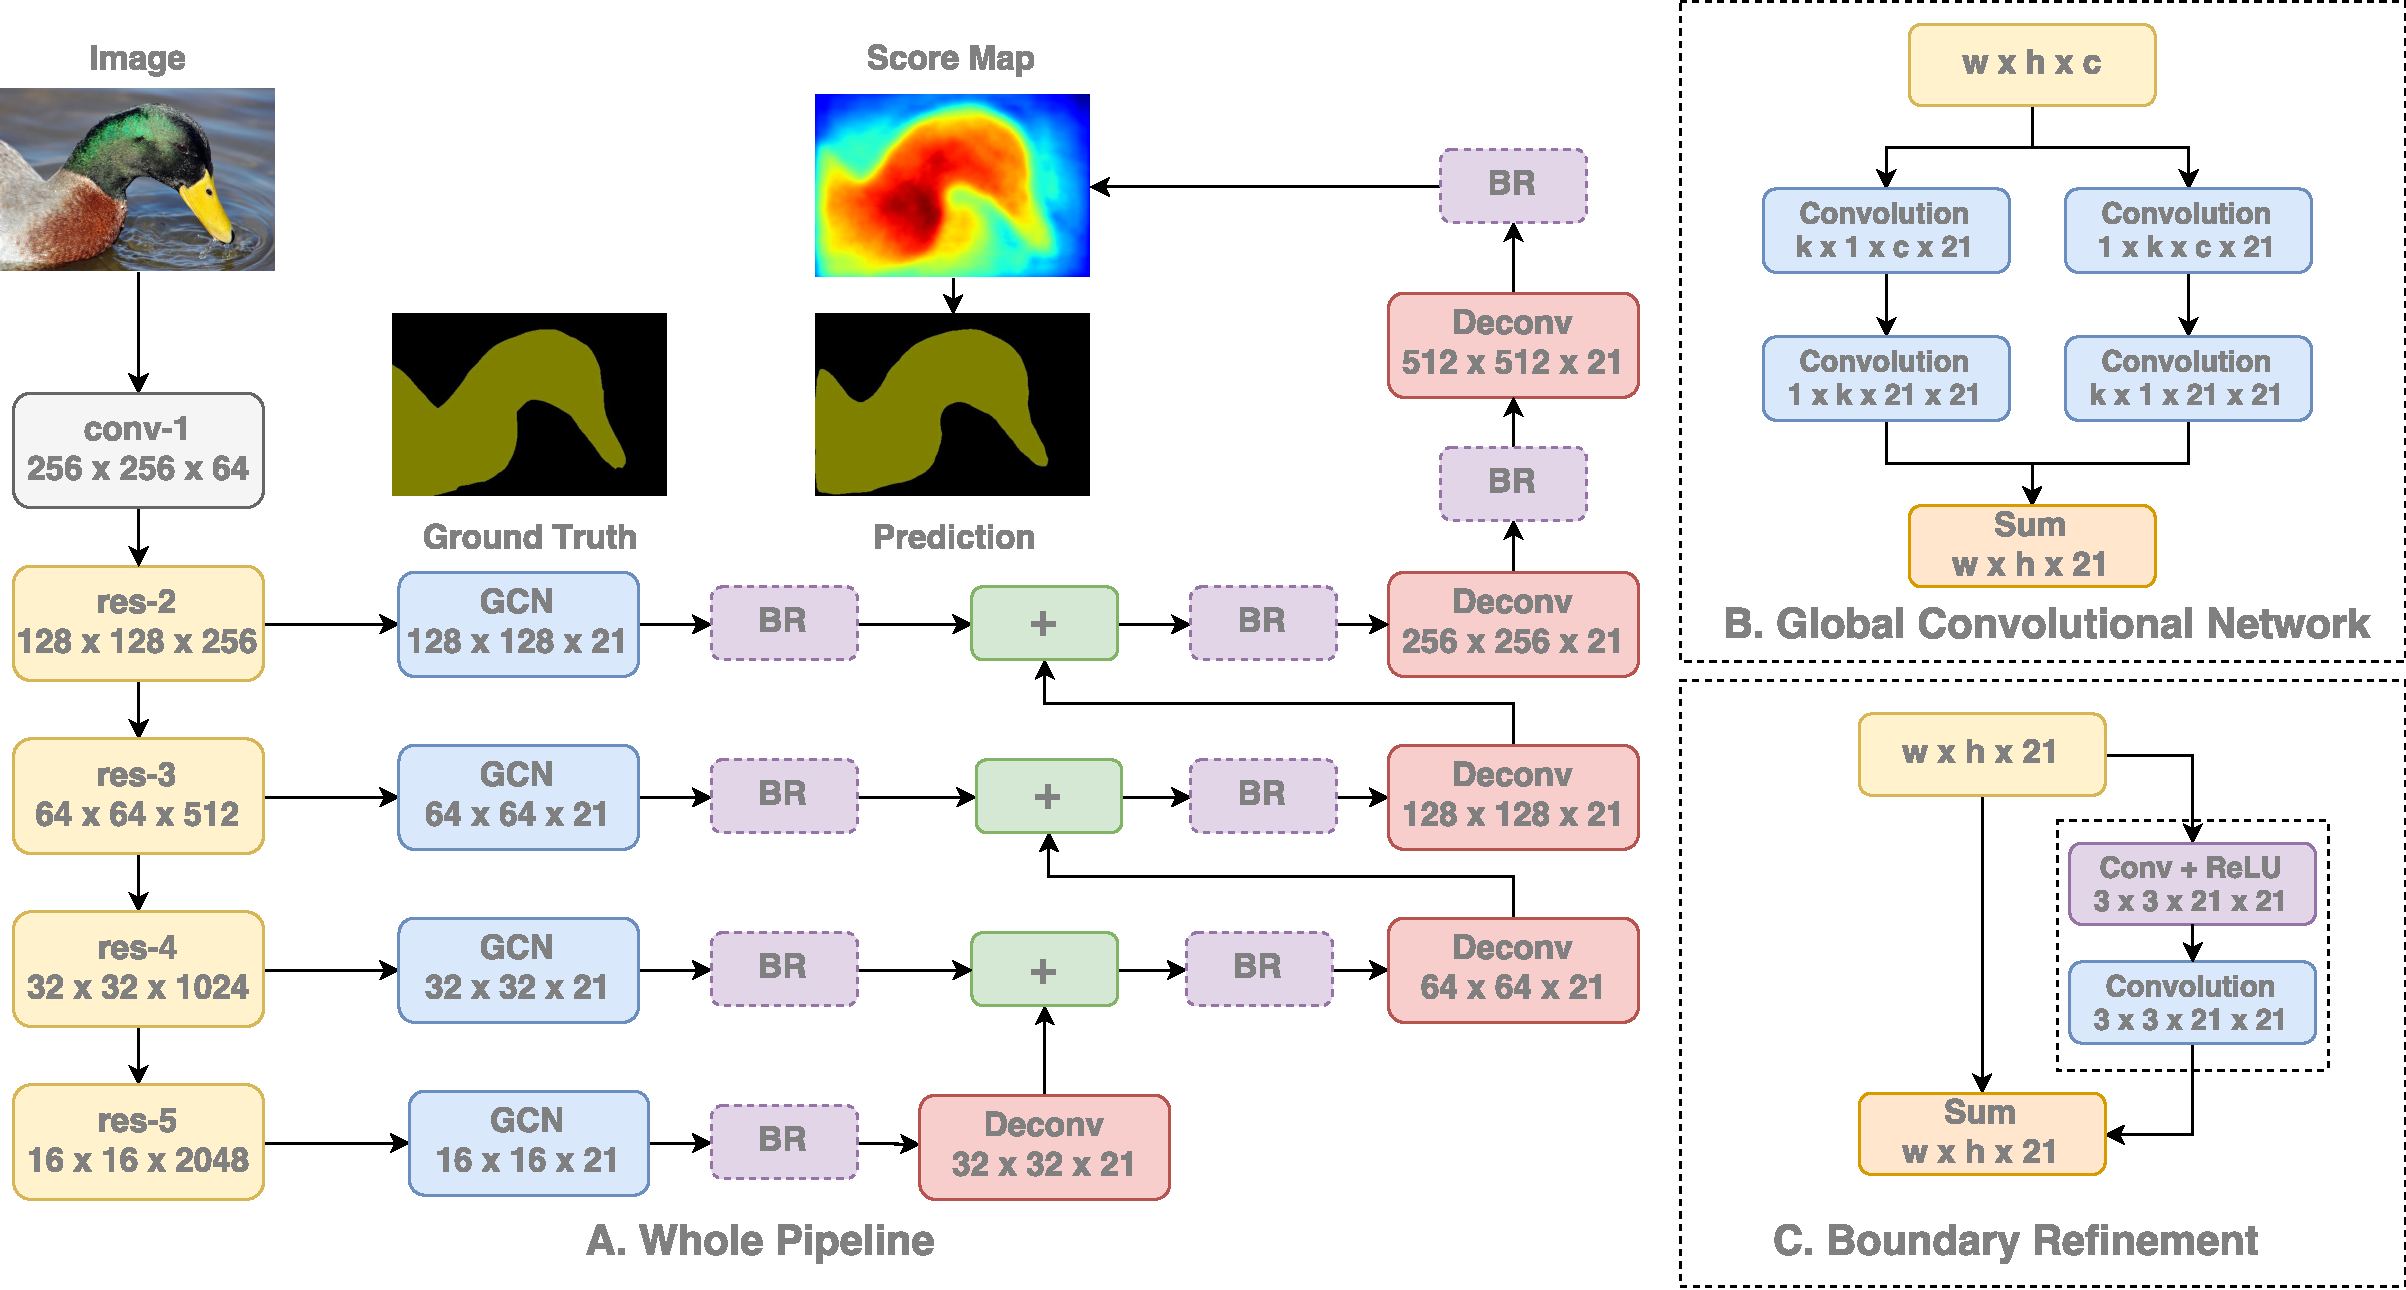
\includegraphics[width=0.95\linewidth]{GCN-network}}

\paragraph{总结1}
GCN(Global Convolution network)能够增大感受野;大的可分离卷积是一种有效的增大感受野方式。

\paragraph{Motivation 2}
GCN中的大卷积核计算量更大,而全局池化(Global Pooling)计算量更小的同时也能获得全局Context。
大的感受野并不意味着能够获取更好的Context,因此可以使用attention策略自适应地整合特征,有所侧重。

\paragraph{解决办法探索2:DFN(CVPR2018)\cite{DFN}}
Backbone使用ResNet。
Head分为smooth network和border network两部分,前者使用global pooling获得更大感受野,并使用CAB(channel attention block)进行加权自适应地整合全局特征;
后者则使用RRB(Refinement Residual Block)获得更好的边缘信息。消融实验结果证明RRB、GP、CAB和DS(deep supervision)都有一定涨点。

{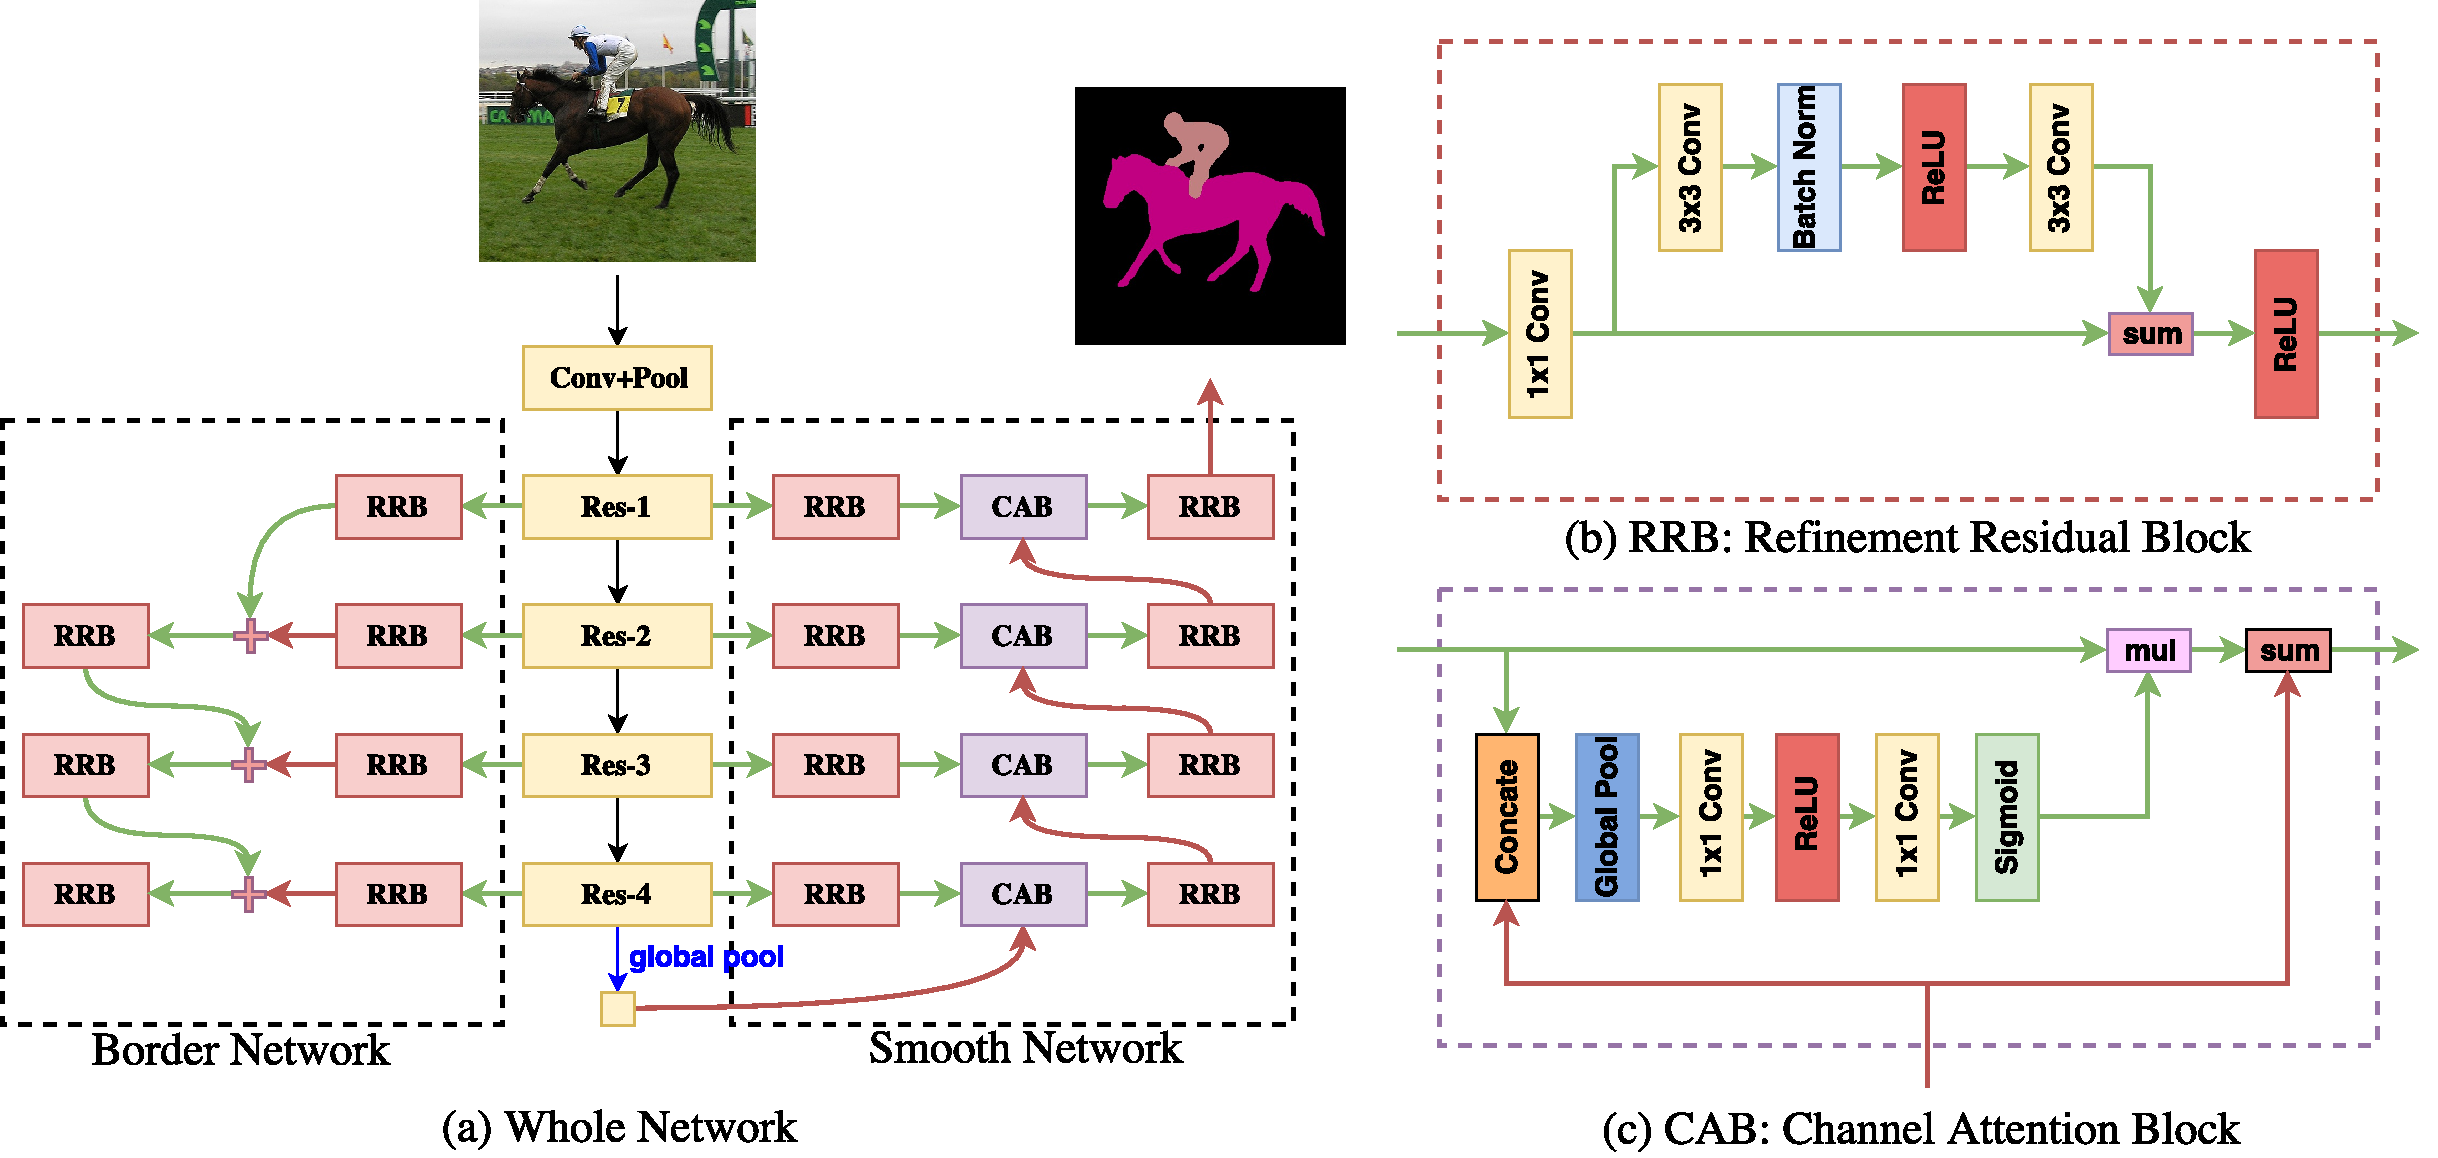
\includegraphics[width=0.95\linewidth]{DFN-network}}

\paragraph{总结2}
Global pooling对于捕获大范围的Context比较有效;使用attention策略进行自适应调整特征权重进行特征整合。
在这里的context包括感受野和特征整合两部分。
代码实现见\cite{torchseg_code}。

\subsubsection{Loss}

\paragraph{Motivation}
全景分割中的thing可能对于stuff的预测有一定的帮助。

\paragraph{解决办法探索:OANet\cite{Panoptic_Megvii}}

三层的监督信号:objects、semantic、stuff,目标是为了优化stuff的结果,通过semantic和stuff一起来预测stuff。

{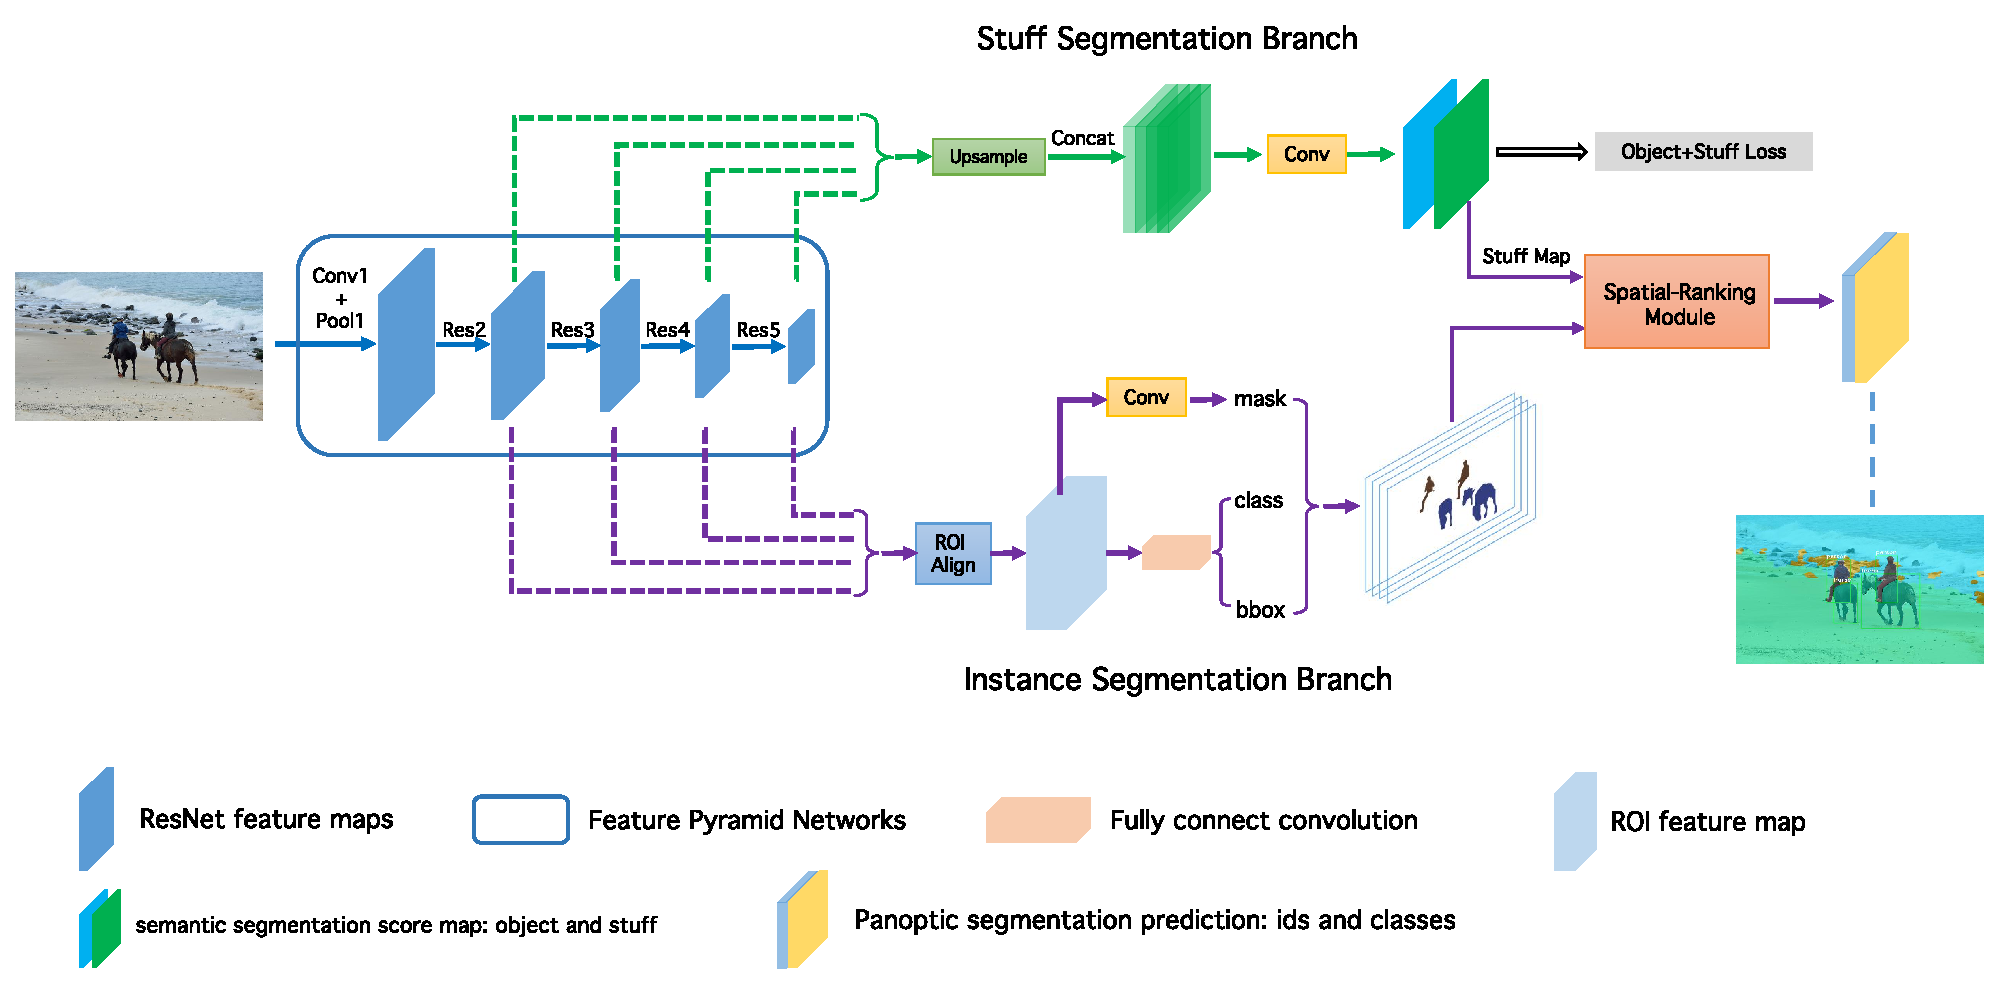
\includegraphics[width=0.95\linewidth]{OANet-network}}

\paragraph{总结}
thing和stuff具有相辅相成的互补效果。
loss是一种不增加计算代价的有效编码context的方式。

\subsection{总结}
\paragraph{不同part的Context} 在Backbone、Head和Loss部分
\paragraph{Context的解释} 更大的感受野Large receptive field、语义分支A semantic branch、空间/特征整合Spatial/feature aggregation
\paragraph{未来工作方向} 明确定义Context;全景分割(Stuff + Thing)
\paragraph{Q$\&$A}
1. boundary refinement 模块:使用一个类res block模块学习残差信息加上本身网络学习到的信息进行边界修复,这只是一个理想中的状态,并不是真正显式的表示出来boundary。
2. stuff和thing的区别

%%%%%%%%%%%%%%%%%%%%%%%%%%%%%%%%%%%%%%%%%%%%%%%%%%%%%%%%%%%%%%%%%%%%%%%%%%%%%%%%
%%% PSANet && UPSNet
%%%%%%%%%%%%%%%%%%%%%%%%%%%%%%%%%%%%%%%%%%%%%%%%%%%%%%%%%%%%%%%%%%%%%%%%%%%%%%%%
\section{Pixel-Level Image Understanding}

%%%%%%%%%%%%%%%%%%%%%%%%%%%%%%%%%%%%%%%%%%%%%%%%%%%%%%%%%%%%%%%%%%%%%%%%%%%%%%%%
\subsection{介绍}

\paragraph{报告嘉宾}赵恒爽 (The Chinese University of Hong Kong)

\paragraph{报告时间}2019年5月29日(星期三)晚上20:00(北京时间)

\paragraph{报告题目}Pixel-Level Image Understanding with Semantic Segmentation and Panoptic Segmentation

\paragraph{报告人简介}
Hengshuang Zhao is currently a fourth year Ph.D. student at The Chinese University of Hong Kong, supervised by Prof. Jiaya Jia. 
Before that, he received the B.E. degree from Huazhong University of Science and Technology in 2015. 
His general research interests cover the broad area of computer vision and deep learning, with special emphasis on high-level image recognition and pixel-level image understanding. 
He and his team won 1st places in ImageNet Scene Parsing Challenge 2016, LSUN Semantic Segmentation Challenge 2017 and WAD Drivable Area Segmentation Challenge 2018. 
Part of his research projects are supported by SenseTime, Adobe, Uber and Intel. His works have been cited for about 1200 times.
个人主页\cite{Hengshuang}。

\paragraph{报告摘要}
Pixel-Level image understanding is a fundamental while challenging task in computer vision. It predicts dense values for all pixels in the image, and is regarded as a very important task that can help achieve a deep understanding of scene, objects, and human. In this talk, I will mainly cover the topics of semantic segmentation and panoptic segmentation. For each topic, I will first go through recent deep learning based approaches and then detail our latest efforts with Point-wise Spatial Attention Network (PSANet) for semantic segmentation and Unified Panoptic Segmentation Network (UPSNet) for panoptic segmentation. Finally, I will discuss some existing problems and the remaining challenges.

\subsection{Semantic Segmentation}

\subsubsection{方法技巧survey}

\paragraph{Semantic Segmentation Dataset}
PASCAL VOC 2012, ADE20K, KITTI, Cityscapes

\paragraph{Fully Convolutional Network}
FCN [Long et al. 2015]

\paragraph{Conditional Random Field}
条件随机场\\
DeepLabV1 [Chen et al. 2015], DPN [Liu et al. 2015], CRF-RNN [Zheng et al. 2015]

\paragraph{Encoder-Decoder}
编码器-解码器模型\\
UNet [Ronneberger et al. 2015], DeconvNet [Noh et al. 2015],
SegNet [Badrinarayanan et al. 2015], LRR [Ghiasi et al. 2016],
RefineNet [Lin et al. 2017], FRRN [Pohlen et al. 2017]

\paragraph{Atrous Convolution / Dilated Convolution}
空洞卷积\\
DeepLabV1 [Chen et al. 2015], Dilation [Fisher et al. 2016]

\paragraph{Context Aggregation}
上下文信息聚合\\
Pooling: ParseNet [Liu et al. 2015], PSPNet [Zhao et al. 2017], DeepLabV2 [Chen et al. 2016]\\
Large Kernel: GCN [Peng et al. 2017]

\paragraph{Neural Architecture Search}
神经网络搜索NAS\\
Search for head: DPC [Chen et al. 2018] \\
Search for backbone: Auto-DeepLab [Liu et al. 2019]

\paragraph{Attention Mechanism}
注意力机制\\
Channel reweighting: SENet [Hu et al. 2018],EncNet [Zhang et al. 2018], DFN [Yu et al. 2018]\\
Spatial attention (dot product): Transformer [Vaswani et al. 2017], Non-Local-Net [Wang et al. 2018], OCNet [Yuan et al. 2018], DANet [Fu et al. 2018], CCNet [Huang et al. 2018]

\subsubsection{新网络探索}

使用PSA网络进行context信息整合;使用auxiliary loss进行deep supervision

{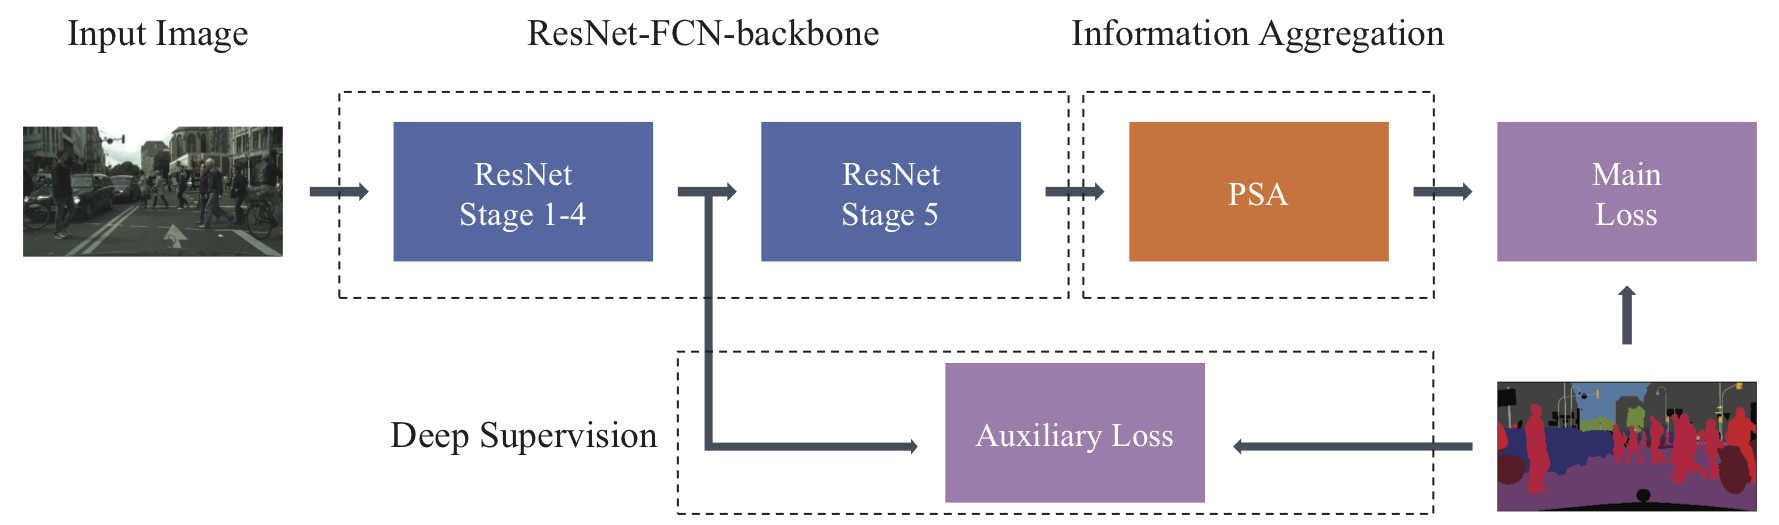
\includegraphics[width=0.95\linewidth]{PSANet-network}}

逐点空间注意网络(PSANet\cite{PSANet})
\begin{itemize}
    \item Conv&Dilated Conv:固定网格,信息流限制在局部区域内
    \item 池化操作:在每个位置固定权重,没有自适应方式
    \item 特征关联:忽略相对位置信息
    \item 逐点空间注意力:用于密集预测的长程上下文聚合,双向信息传播,自适应学习和位置敏感的掩模
\end{itemize}
分为上方的Information collection branch和下方的Information distribution branch两个分支,
collection分支获得的是对当前点有影响的周围context内容,distribution分支获得的是当前的对周围点context提取的影响。
代码实现见\cite{semseg_code}。

{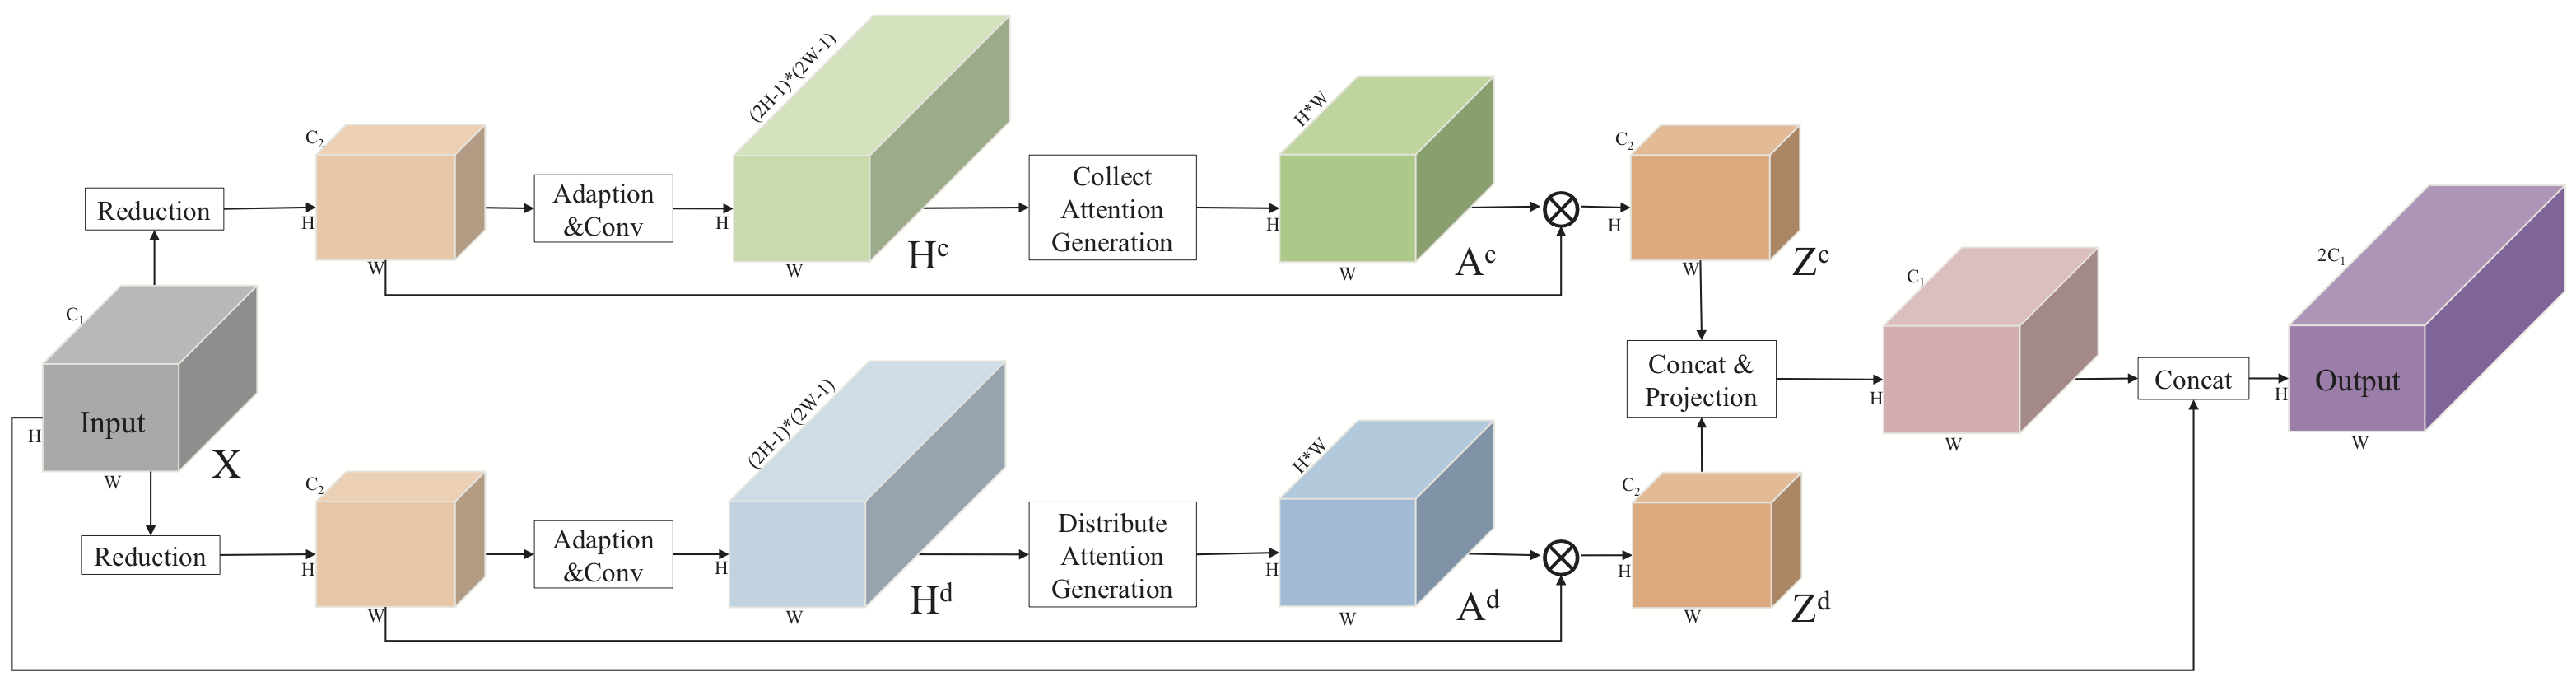
\includegraphics[width=0.95\linewidth]{PSANet-module}}

\subsection{Panoptic Segmentation}

\subsubsection{全景分割介绍}

\paragraph{几种分割方式的比较}
semantic vs instance vs panoptic segmentation: \\
semantic segmentation: instances indistinguishable 同一类别的实例之间无法区分\\
instance segmentation: stuff unsolved 背景stuff无法识别\\
panoptic segmentation: stuff and things are solved, instances distinguishable

\subsubsection{全景分割网络UPSNet\cite{UPSNet}}

\paragraph{要解决的问题}
启发式融合semantic和instance分割结果的问题\\
Heuristic Combination:
semantic分支和instance分支存在计算冗余,heuristic merge不能end-to-end训练\\
Unified Panoptic Segmentation Network (UPSNet):
backbone部分共用减少计算量,head部分使用pixel-wise分类保证了估计的一致性。\\
代码实现见\cite{upsnet_code}。

\paragraph{两种head}
Semantic $\&$ Instance Head\\
Semantic Head: FPN with Deformable Conv\\
Instance Head: Same as Mask-RCNN\\
Panoptic Head: Mask logits from Instance head; Thing $\&$ Stuff logits from Semantic head\\

{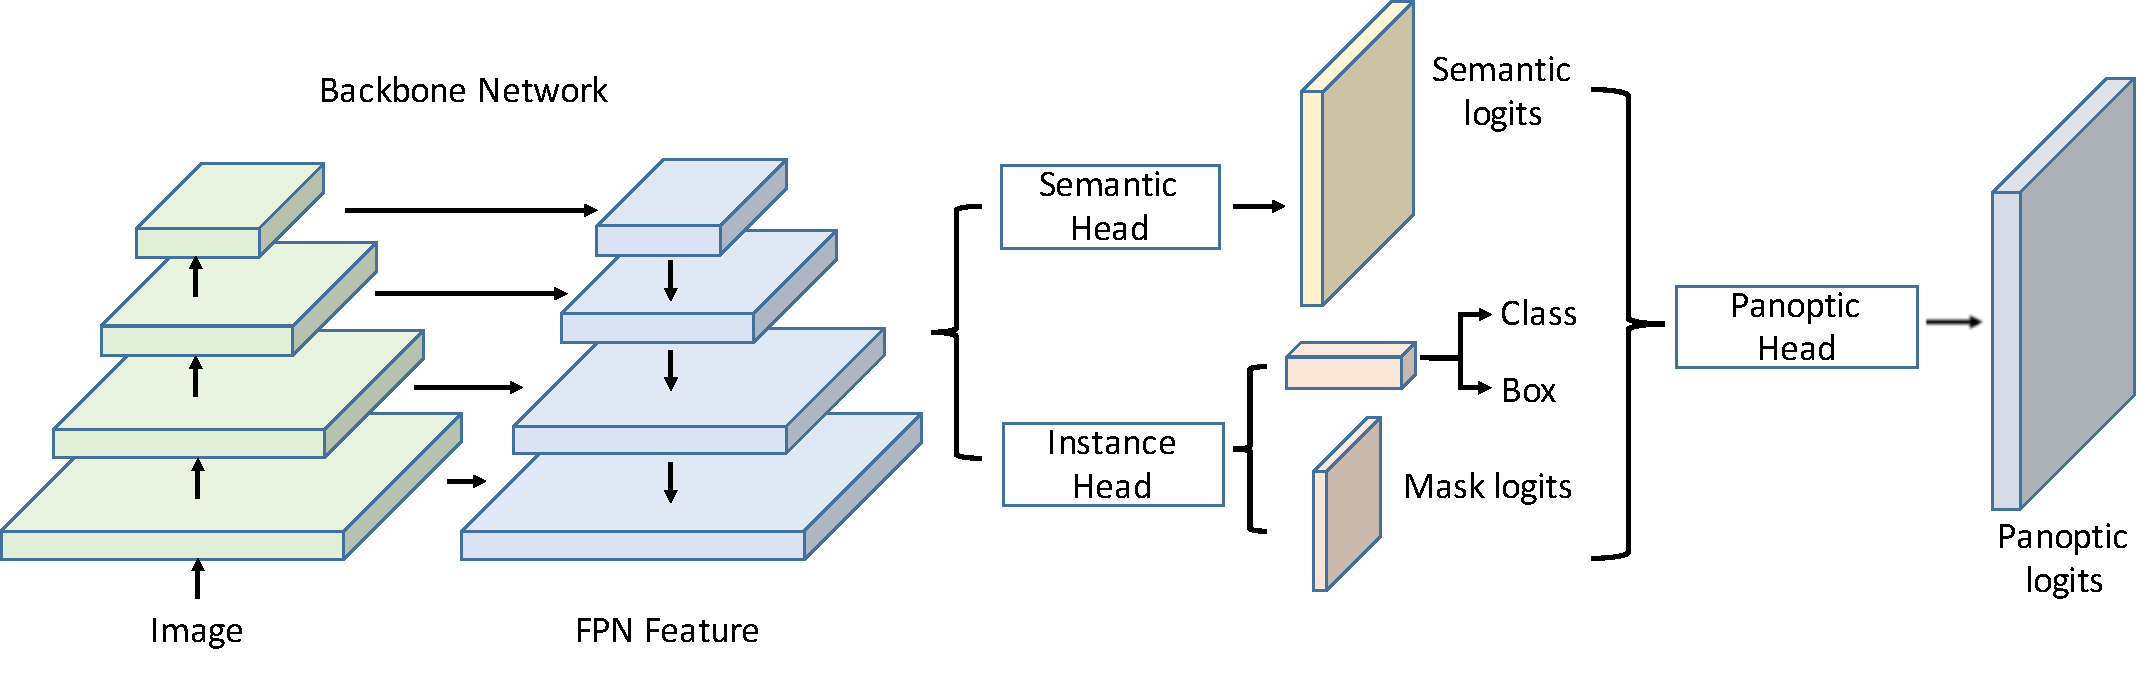
\includegraphics[width=0.95\linewidth]{UPSNet-network}}

\renewcommand\refname{参考文献}
\begin{thebibliography}{99}
    \bibitem[1]{GCN} Large Kernel Matters -- Improve Semantic Segmentation by Global Convolutional Network, Chao Peng, Xiangyu Zhang, Gang Yu, Guiming Luo, Jian Sun,CVPR, 2017
    \bibitem[2]{DFN} Learning a Discriminative Feature Network for Semantic Segmentation, Changqian Yu, Jingbo Wang, Chao Peng, Changxin Gao, Gang Yu, Nong Sang, CVPR, 2018
    \bibitem[3]{BiSeNet} BiSeNet: Bilateral Segmentation Network for Real-time Semantic Segmentation, Changqian Yu, Jingbo Wang, Chao Peng, Changxin Gao, Gang Yu, Nong Sang, ECCV, 2018
    \bibitem[4]{Panoptic_Megvii} http://presentations.cocodataset.org/ECCV18/COCO18-Panoptic-Megvii.pdf
    \bibitem[5]{pspnet} Pyramid Scene Parsing Network, CVPR 2017. Hengshuang Zhao, Jianping Shi, Xiaojuan Qi, Xiaogang Wang, Jiaya Jia.
    \bibitem[6]{ICNet} ICNet for Real - Time Semantic Segmentation on High - Resolution Images, ECCV 2018. Hengshuang Zhao, Xiaojuan Qi, Xiaoyong Shen, Jianping Shi, Jiaya Jia.
    \bibitem[7]{PSANet} PSANet: Point - wise Spatial Attention Network for Scene Parsing, ECCV 2018. Hengshuang Zhao, Yi Zhang, Shu Liu, Jianping Shi, Chen Change Loy, Dahua Lin, Jiaya Jia.
    \bibitem[8]{UPSNet} UPSNet: A Unified Panoptic Segmentation Network, CVPR 2019. Yuwen Xiong, Renjie Liao, Hengshuang Zhao, Rui Hu, Min Bai, Ersin Yumer, Raquel Urtasun.
    \bibitem[9]{Hengshuang} https://hszhao.github.io/
    \bibitem[10]{Gangyu} http://www.skicyyu.org/
    \bibitem[11]{slides} http://valser.org/article-320-1.html
    \bibitem[12]{torchseg_code} https://github.com/ycszen/TorchSeg
    \bibitem[13]{semseg_code} https://github.com/hszhao/semseg
    \bibitem[14]{upsnet_code} https://github.com/uber-research/UPSNet
\end{thebibliography}
\bibliography{BiBTex}

\ifx\allfiles\undefined
\end{document}
\fi